% ============================================================
% Question Bank: ch05-02 Solving Two-Step Equations
% Topic Title: Solving Two-Step Equations
% CCSS: 7.EE.B.4a
% Questions: 27 (15 MC + 6 SA + 6 Graphical)
% ============================================================

% --- Multiple Choice Questions (15) ---

\begin{practiceQuestion}{5-2-q01}{mc}
\begin{questionText}
Solve $4x + 11 = 35$.
\end{questionText}
\choiceA{$x = 6$}
\choiceB{$x = 11.5$}
\choiceC{$x = 8$}
\choiceD{$x = 46$}
\correctAnswer{A}
\explanation{Subtract $11$: $4x = 24$. Divide by $4$: $x = 6$. Check: $4(6) + 11 = 24 + 11 = 35$ \checkmark.}
\end{practiceQuestion}

\begin{practiceQuestion}{5-2-q02}{mc}
\begin{questionText}
Solve $7n - 15 = 41$.
\end{questionText}
\choiceA{$n = 4$}
\choiceB{$n = 8$}
\choiceC{$n = 3.71$}
\choiceD{$n = 56$}
\correctAnswer{B}
\explanation{Add $15$: $7n = 56$. Divide by $7$: $n = 8$. Check: $7(8) - 15 = 56 - 15 = 41$ \checkmark.}
\end{practiceQuestion}

\begin{practiceQuestion}{5-2-q03}{mc}
\begin{questionText}
What is the value of $y$ in $\dfrac{y}{5} + 8 = 14$?
\end{questionText}
\choiceA{$y = 110$}
\choiceB{$y = 10$}
\choiceC{$y = 30$}
\choiceD{$y = 1.2$}
\correctAnswer{C}
\explanation{Subtract $8$: $\frac{y}{5} = 6$. Multiply by $5$: $y = 30$. Check: $\frac{30}{5} + 8 = 6 + 8 = 14$ \checkmark.}
\end{practiceQuestion}

\begin{practiceQuestion}{5-2-q04}{mc}
\begin{questionText}
Solve $-6x + 14 = -4$.
\end{questionText}
\choiceA{$x = -3$}
\choiceB{$x = 3$}
\choiceC{$x = -\dfrac{5}{3}$}
\choiceD{$x = 10$}
\correctAnswer{B}
\explanation{Subtract $14$: $-6x = -18$. Divide by $-6$: $x = 3$. Check: $-6(3) + 14 = -18 + 14 = -4$ \checkmark.}
\end{practiceQuestion}

\begin{practiceQuestion}{5-2-q05}{mc}
\begin{questionText}
What is the first step to solve $\dfrac{x}{8} - 5 = 7$?
\end{questionText}
\choiceA{Multiply both sides by $8$}
\choiceB{Subtract $5$ from both sides}
\choiceC{Add $5$ to both sides}
\choiceD{Divide both sides by $8$}
\correctAnswer{C}
\explanation{To undo the subtraction of $5$, add $5$ to both sides first: $\frac{x}{8} = 12$.}
\end{practiceQuestion}

\begin{practiceQuestion}{5-2-q06}{mc}
\begin{questionText}
Solve $19 = 3m + 7$.
\end{questionText}
\choiceA{$m = 4$}
\choiceB{$m = 8\frac{2}{3}$}
\choiceC{$m = 6$}
\choiceD{$m = 12$}
\correctAnswer{A}
\explanation{Subtract $7$: $12 = 3m$. Divide by $3$: $m = 4$. Check: $3(4) + 7 = 12 + 7 = 19$ \checkmark.}
\end{practiceQuestion}

\begin{practiceQuestion}{5-2-q07}{mc}
\begin{questionText}
A streaming service costs $\$8$ per month plus a $\$15$ activation fee. Tanya paid $\$79$ total. How many months did she subscribe?
\end{questionText}
\choiceA{$8$ months}
\choiceB{$9$ months}
\choiceC{$7$ months}
\choiceD{$10$ months}
\correctAnswer{A}
\explanation{$8m + 15 = 79$. Subtract $15$: $8m = 64$. Divide by $8$: $m = 8$.}
\end{practiceQuestion}

\begin{practiceQuestion}{5-2-q08}{mc}
\begin{questionText}
Solve $\dfrac{n}{9} - 4 = 2$.
\end{questionText}
\choiceA{$n = 18$}
\choiceB{$n = 54$}
\choiceC{$n = -18$}
\choiceD{$n = 6$}
\correctAnswer{B}
\explanation{Add $4$: $\frac{n}{9} = 6$. Multiply by $9$: $n = 54$. Check: $\frac{54}{9} - 4 = 6 - 4 = 2$ \checkmark.}
\end{practiceQuestion}

\begin{practiceQuestion}{5-2-q09}{mc}
\begin{questionText}
Which equation has the solution $x = -3$?
\end{questionText}
\choiceA{$5x + 10 = -5$}
\choiceB{$5x + 10 = 25$}
\choiceC{$5x - 10 = -5$}
\choiceD{$5x + 3 = -10$}
\correctAnswer{A}
\explanation{Substitute $x = -3$: $5(-3) + 10 = -15 + 10 = -5$. So $5x + 10 = -5$ is correct.}
\end{practiceQuestion}

\begin{practiceQuestion}{5-2-q10}{mc}
\begin{questionText}
Solve $-7k + 21 = 0$.
\end{questionText}
\choiceA{$k = -3$}
\choiceB{$k = 0$}
\choiceC{$k = 3$}
\choiceD{$k = 21$}
\correctAnswer{C}
\explanation{Subtract $21$: $-7k = -21$. Divide by $-7$: $k = 3$. Check: $-7(3) + 21 = -21 + 21 = 0$ \checkmark.}
\end{practiceQuestion}

\begin{practiceQuestion}{5-2-q11}{mc}
\begin{questionText}
You have $\$90$ in savings. You spend $\$11$ per week. After how many weeks will you have $\$2$ left?
\end{questionText}
\choiceA{$7$ weeks}
\choiceB{$9$ weeks}
\choiceC{$8$ weeks}
\choiceD{$6$ weeks}
\correctAnswer{C}
\explanation{$90 - 11w = 2$. Subtract $90$: $-11w = -88$. Divide by $-11$: $w = 8$.}
\end{practiceQuestion}

\begin{practiceQuestion}{5-2-q12}{mc}
\begin{questionText}
A student solved $6x + 18 = 42$ and got $x = 10$. What error did the student most likely make?
\end{questionText}
\choiceA{Forgot to subtract $18$}
\choiceB{Added $18$ instead of subtracting}
\choiceC{Divided by $6$ before subtracting $18$}
\choiceD{Subtracted $18$ from the left side only}
\correctAnswer{B}
\explanation{If the student added $18$: $6x = 60$, then $x = 10$. The correct step is to subtract $18$: $6x = 24$, $x = 4$.}
\end{practiceQuestion}

\begin{practiceQuestion}{5-2-q13}{mc}
\begin{questionText}
Solve $-3x - 11 = 10$.
\end{questionText}
\choiceA{$x = -7$}
\choiceB{$x = 7$}
\choiceC{$x = -\dfrac{1}{3}$}
\choiceD{$x = \dfrac{1}{3}$}
\correctAnswer{A}
\explanation{Add $11$: $-3x = 21$. Divide by $-3$: $x = -7$. Check: $-3(-7) - 11 = 21 - 11 = 10$ \checkmark.}
\end{practiceQuestion}

\begin{practiceQuestion}{5-2-q14}{mc}
\begin{questionText}
Solve $15 = \dfrac{x}{4} + 3$.
\end{questionText}
\choiceA{$x = 72$}
\choiceB{$x = 48$}
\choiceC{$x = 3$}
\choiceD{$x = 12$}
\correctAnswer{B}
\explanation{Subtract $3$: $12 = \frac{x}{4}$. Multiply by $4$: $x = 48$. Check: $\frac{48}{4} + 3 = 12 + 3 = 15$ \checkmark.}
\end{practiceQuestion}

\begin{practiceQuestion}{5-2-q15}{mc}
\begin{questionText}
Solve $8p + 5 = -19$.
\end{questionText}
\choiceA{$p = -3$}
\choiceB{$p = 3$}
\choiceC{$p = -\dfrac{7}{4}$}
\choiceD{$p = -1.75$}
\correctAnswer{A}
\explanation{Subtract $5$: $8p = -24$. Divide by $8$: $p = -3$. Check: $8(-3) + 5 = -24 + 5 = -19$ \checkmark.}
\end{practiceQuestion}

% --- Short Answer Questions (6) ---

\begin{practiceQuestion}{5-2-q16}{sa}
\begin{questionText}
Solve $3x + 22 = 40$.
\end{questionText}
\correctAnswer{$x = 6$}
\explanation{Subtract $22$: $3x = 18$. Divide by $3$: $x = 6$. Check: $3(6) + 22 = 18 + 22 = 40$ \checkmark.}
\end{practiceQuestion}

\begin{practiceQuestion}{5-2-q17}{sa}
\begin{questionText}
Solve $\dfrac{y}{6} - 7 = 5$.
\end{questionText}
\correctAnswer{$y = 72$}
\explanation{Add $7$: $\frac{y}{6} = 12$. Multiply by $6$: $y = 72$. Check: $\frac{72}{6} - 7 = 12 - 7 = 5$ \checkmark.}
\end{practiceQuestion}

\begin{practiceQuestion}{5-2-q18}{sa}
\begin{questionText}
Solve $-9n + 5 = -31$.
\end{questionText}
\correctAnswer{$n = 4$}
\explanation{Subtract $5$: $-9n = -36$. Divide by $-9$: $n = 4$. Check: $-9(4) + 5 = -36 + 5 = -31$ \checkmark.}
\end{practiceQuestion}

\begin{practiceQuestion}{5-2-q19}{sa}
\begin{questionText}
A pet groomer charges $\$18$ per dog plus a $\$10$ supply fee. She earned $\$100$ today. How many dogs did she groom?
\end{questionText}
\correctAnswer{$5$ dogs}
\explanation{$18d + 10 = 100$. Subtract $10$: $18d = 90$. Divide by $18$: $d = 5$.}
\end{practiceQuestion}

\begin{practiceQuestion}{5-2-q20}{sa}
\begin{questionText}
Solve $120 - 8x = 24$.
\end{questionText}
\correctAnswer{$x = 12$}
\explanation{Subtract $120$: $-8x = -96$. Divide by $-8$: $x = 12$. Check: $120 - 8(12) = 120 - 96 = 24$ \checkmark.}
\end{practiceQuestion}

\begin{practiceQuestion}{5-2-q21}{sa}
\begin{questionText}
Solve $17 = 5x - 8$.
\end{questionText}
\correctAnswer{$x = 5$}
\explanation{Add $8$: $25 = 5x$. Divide by $5$: $x = 5$. Check: $5(5) - 8 = 25 - 8 = 17$ \checkmark.}
\end{practiceQuestion}

% --- Graphical MC Questions (3) ---

\begin{practiceQuestion}{5-2-q22}{gmc}
\begin{questionText}
Look at the balance scale. Both sides are equal. What is the value of $x$?

\begin{center}
\begin{tikzpicture}[scale=0.84]
  % Fulcrum
  \draw[thick] (0,-0.5) -- (-0.4,-1.2) -- (0.4,-1.2) -- cycle;
  % Beam
  \draw[thick] (-5,0) -- (5,0);
  % Left pan
  \draw[thick] (-5,0) -- (-5.8,-0.7) -- (-4.2,-0.7) -- (-5,0);
  \draw[thick,fill=funBlue!20] (-5.8,-0.7) -- (-5.8,-1.05) -- (-4.2,-1.05) -- (-4.2,-0.7) -- cycle;
  % Left: 3x + 9
  \node[draw,fill=funBlue!40,minimum width=0.42cm,minimum height=0.42cm] at (-5.45,-1.48) {\small $x$};
  \node[draw,fill=funBlue!40,minimum width=0.42cm,minimum height=0.42cm] at (-5.00,-1.48) {\small $x$};
  \node[draw,fill=funBlue!40,minimum width=0.42cm,minimum height=0.42cm] at (-4.55,-1.48) {\small $x$};
  \node at (-5.38,-1.98) {\small $+$};
  \node[draw,fill=funOrange!35,minimum width=0.78cm,minimum height=0.5cm] at (-4.96,-1.98) {\small $9$};
  % Right pan
  \draw[thick] (5,0) -- (5.8,-0.7) -- (4.2,-0.7) -- (5,0);
  \draw[thick,fill=funOrange!20] (5.8,-0.7) -- (5.8,-1.05) -- (4.2,-1.05) -- (4.2,-0.7) -- cycle;
  \node at (5,-0.88) {\small $42$};
\end{tikzpicture}
\end{center}
\end{questionText}
\choiceA{$x = 11$}
\choiceB{$x = 14$}
\choiceC{$x = 17$}
\choiceD{$x = 33$}
\correctAnswer{A}
\explanation{The balance gives $3x + 9 = 42$. Subtract $9$: $3x = 33$. Divide by $3$: $x = 11$.}
\end{practiceQuestion}

\begin{practiceQuestion}{5-2-q23}{gmc}
\begin{questionText}
Use the function table to find the value of $x$ when the output is $31$.

\begin{center}
\begin{tabular}{|c|c|}
\hline
\textbf{Input ($x$)} & \textbf{Output} \\
\hline
$1$ & $7$ \\
\hline
$2$ & $11$ \\
\hline
$3$ & $15$ \\
\hline
$?$ & $31$ \\
\hline
\end{tabular}
\end{center}
\end{questionText}
\choiceA{$x = 6$}
\choiceB{$x = 7$}
\choiceC{$x = 8$}
\choiceD{$x = 9$}
\correctAnswer{B}
\explanation{The pattern is $4x + 3$. Set $4x + 3 = 31$. Subtract $3$: $4x = 28$. Divide by $4$: $x = 7$.}
\end{practiceQuestion}

\begin{practiceQuestion}{5-2-q24}{gmc}
\begin{questionText}
A rectangle has an area of $78$ square inches. What is the value of $x$?

\begin{center}
\begin{tikzpicture}[scale=0.6]
  \draw[thick,fill=funBlue!10] (0,0) rectangle (6,3);
  \draw[<->] (0,-0.5) -- (6,-0.5);
  \node[below] at (3,-0.5) {$6$ in.};
  \draw[<->] (6.5,0) -- (6.5,3);
  \node[right] at (6.5,1.5) {$(2x + 1)$ in.};
\end{tikzpicture}
\end{center}
\end{questionText}
\choiceA{$x = 6$}
\choiceB{$x = 7$}
\choiceC{$x = 12$}
\choiceD{$x = 13$}
\correctAnswer{A}
\explanation{Area $= 6(2x + 1) = 78$. Divide by $6$: $2x + 1 = 13$. Subtract $1$: $2x = 12$. Divide by $2$: $x = 6$.}
\end{practiceQuestion}

% --- Graphical SA Questions (3) ---

\begin{practiceQuestion}{5-2-q25}{gsa}
\begin{questionText}
The balance scale is in equilibrium. Find the value of $n$.

\begin{center}
\begin{tikzpicture}[scale=0.92]
  % Fulcrum
  \draw[thick] (0,-0.5) -- (-0.4,-1.2) -- (0.4,-1.2) -- cycle;
  % Beam
  \draw[thick] (-5.4,0) -- (5.4,0);
  % Left pan
  \draw[thick] (-5.2,0) -- (-6.25,-0.82) -- (-4.15,-0.82) -- (-5.2,0);
  \draw[thick,fill=funBlue!20] (-6.25,-0.82) -- (-6.25,-1.26) -- (-4.15,-1.26) -- (-4.15,-0.82) -- cycle;
  \node at (-5.2,-1.04) {$5n - 7$};
  % Right pan
  \draw[thick] (5.2,0) -- (6.25,-0.82) -- (4.15,-0.82) -- (5.2,0);
  \draw[thick,fill=funOrange!20] (6.25,-0.82) -- (6.25,-1.26) -- (4.15,-1.26) -- (4.15,-0.82) -- cycle;
  \node at (5.2,-1.04) {$38$};
\end{tikzpicture}
\end{center}
\end{questionText}
\correctAnswer{$n = 9$}
\explanation{The balance gives $5n - 7 = 38$. Add $7$: $5n = 45$. Divide by $5$: $n = 9$. Check: $5(9) - 7 = 38$ \checkmark.}
\end{practiceQuestion}

\begin{practiceQuestion}{5-2-q26}{gsa}
\begin{questionText}
The perimeter of the equilateral triangle below is $57$ cm. Find $x$.

\begin{center}
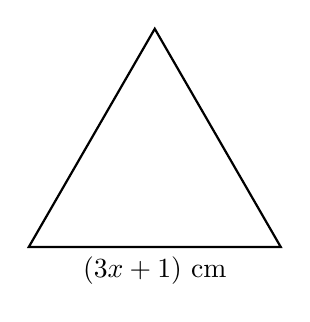
\begin{tikzpicture}[scale=0.8]
  \draw[thick] (0,0) -- (4,0) -- (2,3.464) -- cycle;
  \node[below] at (2,0) {$(3x + 1)$ cm};
\end{tikzpicture}
\end{center}
\end{questionText}
\correctAnswer{$x = 6$}
\explanation{All three sides are equal, so $3(3x + 1) = 57$. Divide by $3$: $3x + 1 = 19$. Subtract $1$: $3x = 18$. Divide by $3$: $x = 6$.}
\end{practiceQuestion}

\begin{practiceQuestion}{5-2-q27}{gsa}
\begin{questionText}
The total distance around the rectangular running track is $320$ meters. Find the width $w$.

\begin{center}
\begin{tikzpicture}[scale=0.5]
  \draw[thick,fill=funBlue!10] (0,0) rectangle (10,4);
  \draw[<->] (0,-0.6) -- (10,-0.6);
  \node[below] at (5,-0.6) {$100$ m};
  \draw[<->] (10.6,0) -- (10.6,4);
  \node[right] at (10.6,2) {$w$ m};
\end{tikzpicture}
\end{center}
\end{questionText}
\correctAnswer{$w = 60$}
\explanation{Perimeter $= 2(100) + 2w = 320$. Simplify: $200 + 2w = 320$. Subtract $200$: $2w = 120$. Divide by $2$: $w = 60$.}
\end{practiceQuestion}
